\section{Evaluation}\label{sec:evaluation}
\begin{figure*}
    \begin{subfigure}[b]{0.25\linewidth}
    \centering 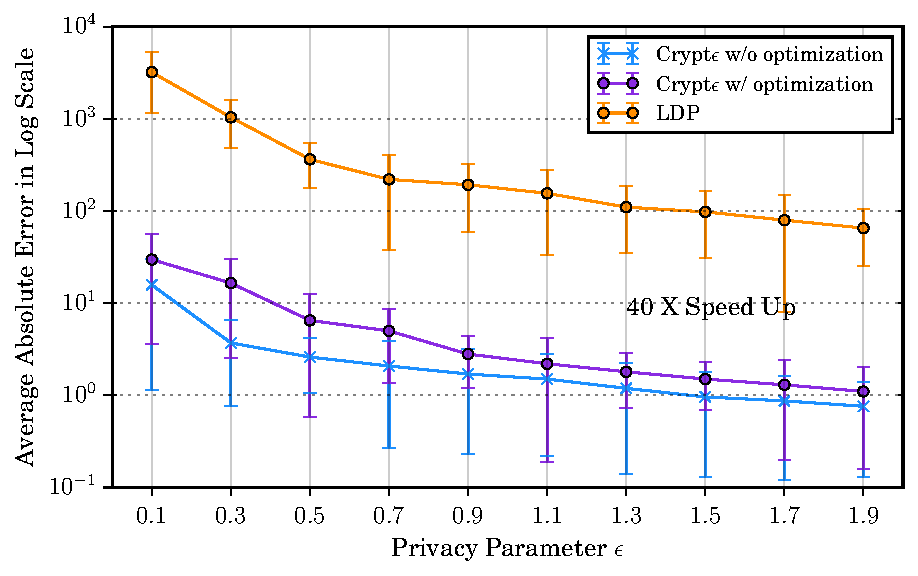
\includegraphics[width=1\linewidth]{t5_final.pdf}
        \caption{Program 5}
        \label{fig:accuracy_p5}\end{subfigure}%%
    \begin{subfigure}[b]{0.25\linewidth}
    \centering    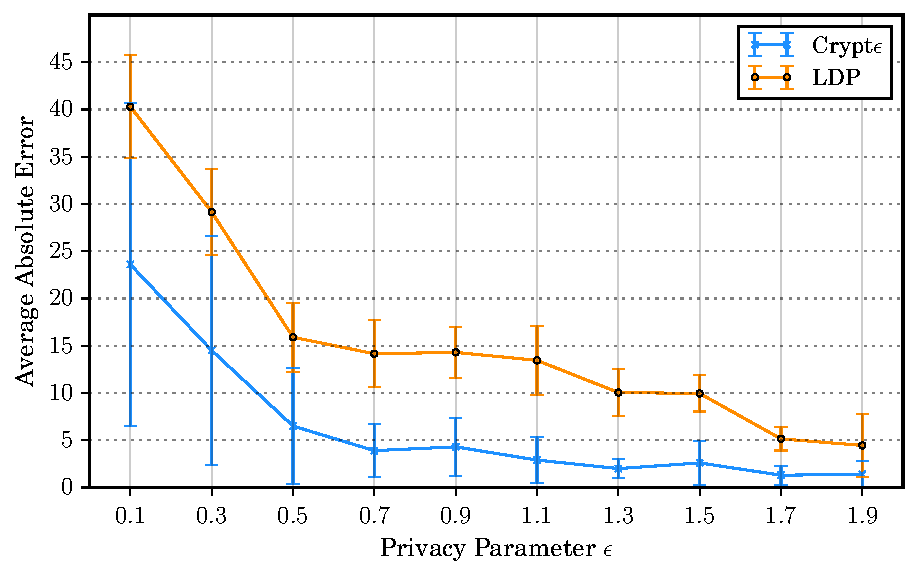
\includegraphics[width=1\linewidth]{t7_final.pdf}
        \caption{ Program 7}
        \label{fig:accuracy_p7}\end{subfigure}%%
      \begin{subfigure}[b]{0.25\linewidth}
    \centering    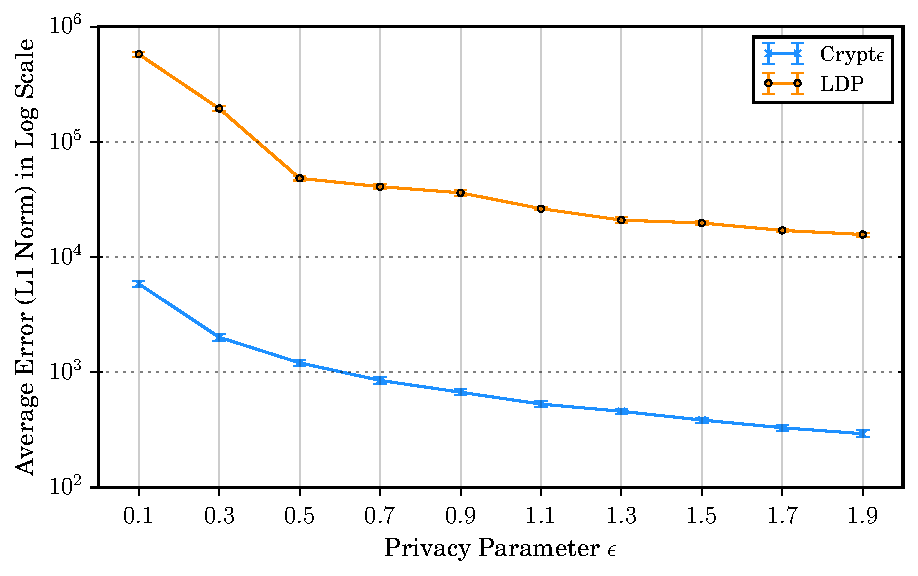
\includegraphics[width=1\linewidth]{t3_final.pdf}
        \caption{Program 3}
        \label{fig:accuracy_p3}
    \end{subfigure}%%
    \begin{subfigure}[b]{0.25\linewidth}
        \centering
         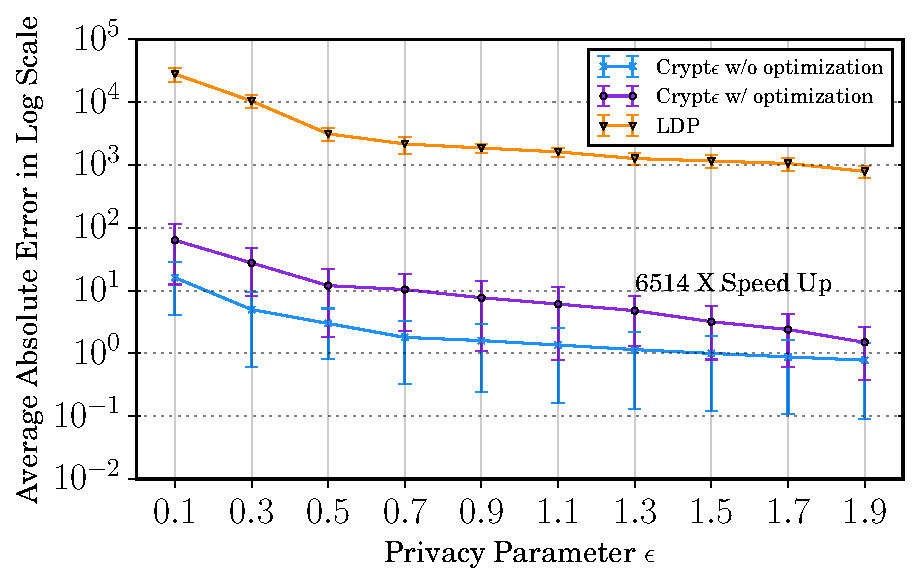
\includegraphics[width=1\linewidth]{t1_final.pdf}
        \caption{ Program 8 \xh{(update plot)}}
        \label{fig:accuracy_p8}
    \end{subfigure}%%
     \caption{Accuracy Evaluation of \system Programs}\label{fig:accuracy}
\end{figure*}

In this section, we experimentally evaluate \system to answer the following questions: i) Do \system programs have significantly lower error than that for the corresponding state-of-the-art LDP implementations? ii) Is the program execution timing for \system practical? iii) Do the proposed optimizations in \system provide substantial performance improvement over the unoptimized \system? Here are our highlighted results.
\squishlist
\item \system can achieve 2 orders of smaller errors than the existing LDP implementations (Figure~\ref{fig:accuracy}).
\item The performance cost of a large class of \system programs is less than 5 minutes for a data set of 32561 users. The \AS shares more performance cost than the \CPS.  (Table~\ref{tab:time})
\item The optimization techniques in \system can improve the performance of non-optimized \system up to \xh{xx} times (Table~\ref{tab:time}).
\squishend

\subsection{Methodology} \label{sec:methodology}
\stitle{Dataset \& Program:} We evaluated our system and the state-of-the-art LDP implementations~\cite{LDP1} on the Adult dataset from the UCI repository \cite{UCI}  which has been extracted from the 1994 census data. The dataset is of size $32,651$. We considered the programs outlined in Table~\ref{tab:programexamples}. Due to space constraint, we focus on P3,P5,P7,P8, as they  cover all the three classes of interactions between the \AS and the \CPS described in Section~\ref{sec:interactions}.  Results for programs P1, P2, P4 and P6 are presented in \xh{Appendix~\ref{}}.

\stitle{Metrics:}
For the accuracy of a program which outputs a vector, we measure the difference between the true answer $V$ before adding any noise and the noisy answer $\hat{V}$ using the $L_1$-norm, i.e. $\|V-\hat{V}\|_1 = \sum_{i} |V[i]-\hat{V}[i]|$. If the output is a scalar, we report the absolute difference between the noisy answer $\hat{c}$ and the true answer $c$. For the performance of \system programs, we measure the program processing time in seconds. Each program is repeated 10 times. We report the mean and the standard deviation for the error and the performance cost.

\stitle{Configuration:} We implemented \system in python with EMP toolkit~\cite{} and LabHE package~\cite{}. The prototype also includes the optimization techniques described in Section~\ref{sec:optimization} including both DP based optimizations (DP range tree and DP index) and implementation based optimizations (pre-computation and off-line processing). For Adult dataset, \system constructs a DP index optimization over the attribute $NativeCountry$ for programs that use this attribute in the filtering condition (e.g. P4 and P5). Our experiments assign $20\%$ of the program privacy budget towards constructing the index and the remain budget for the program. \system also constructs a DP range tree over the attribute $Age$ with the full privacy budget for programs for a set of range queries on $Age$ (e.g. P8). This is the default implementation for \system.  We refer the implementation without the optimization as the unoptimized \system.
All the programs run on Mac OS. We evaluated our prototype on \xh{xx} servers. The servers each have  32GB of memory, 1TB SSD, and 2.6GHz 6‑core 8th‑generation Intel Core i7 processor.




\eat{
\\\textbf{Programs:}
To answer the aforementioned questions we ran the experiments on 4 of the Crypt$\epsilon$ programs previously outlined in Table 3, namely P1,P3,P5 and P7. In this section we rename P1,P5,P7 and P3 as Program A, Program B, Program C and Program D respectively.  %Each program is compared with the corresponding state-of-the-art \textsf{LDP} implementation \cite{LDP1}.
Additional experimental results for programs P2,P4 and P6 from Table 3 are presented in Appendix.% We rename the examples 5.1,5.2,5.3,5.4,5.6 and 5.7 as P1,P2,P6,. The reason behind this grouping is to arrange the programs in their increasing order of complexity.  %\begin{itemize}\item \textbf{Program 1} - Count the number of records having age in range $[50,60]$ \\\textbf{\textsf{LDP} Competitor} - Frequency oracle of \cite{LDP1} constructed over attribute $Age$. \item \textbf{Program 2} - Report the top 5 most frequent age values. \\\textbf{\textsf{LDP} Competitor} - Frequency oracle of \cite{LDP1} constructed over attribute $Age$.  \item \textbf{Program 3 }- Report the marginal on attributes $Age$ and $Gender$. \\\textbf{\textsf{LDP} Competitor }- Frequency oracle of \cite{LDP1} constructed over attribute $Age \times Gender$. \item \textbf{Program 4 }- Report the marginal on attributes $Age$ and $Gender$ with $NativeCountry=Mexico$\\\textbf{\textsf{LDP} Competitor }- Frequency oracle of \cite{LDP1} constructed over attribute $Age\times Gender \times NativeCountry$. \item \textbf{Program 5 }- Count the number of natively Mexican male employees of age 30.\\\textbf{\textsf{LDP} Competitor }- Frequency oracle of \cite{LDP1} constructed over attribute $Age\times Gender \times NativeCountry$. \item \textbf{Program 6 }- Count the number of distinct age values for male employees. \\\textbf{\textsf{LDP} Competitor }-Frequency oracle of \cite{LDP1} constructed over attribute $Age\times Gender$.% and reports the number of non-zero counts after suitable adjustment for thresholding. 
%\item \textbf{Program 7 }- Count the number of age values with at least 10 records. \\\textbf{\textsf{LDP} Competitor }- Frequency oracle of \cite{LDP1} constructed over attribute $Age$. \end{itemize}
\\\textbf{Dataset:}
We ran our experiments on the Adult dataset from the UCI repository \cite{UCI}  which has been extracted from the 1994 census data. The dataset is of size $32,651$.
\\\textbf{Metrics:}
\\\textbf{\textit{Accuracy:}} For accuracy the following metrics are used
\\$\bullet$ Programs A, B and C use absolute error $ =|c-\hat{c}|$ where $c$ is the true count and $\hat{c}$ is the noisy output.\\ $\bullet$ Programs D uses the $L1-Norm$ error metric given  by $Error=\sum_{i}|V[i]-\hat{V}[i]|, i \in [|V|]$.\\
For each of the programs, we report the mean error values over 10 repetitions.\\
\textbf{\textit{Performance:}} For measuring performance we report the mean total execution time in seconds of each program, over 10 repetitions. 
}

%uses the error measure given by the fraction of age values returned in the top 5 that have value less than $ct_5-\alpha$  where  $ct_5$ is the count of the $5^{th}$ largest value and $\alpha=\frac{1}{\epsilon}\log\frac{1}{\delta}$ is a slack parameter. The slack parameter is required because with probability $1-\delta$ no differentially private algorithm can distinguish between any two counts that differ by less than $\alpha$. We use $\delta=0.05$ for our experiment. \item Programs 3, 4 and 5 \end{itemize}


\subsection{Results}\label{sec:results}
%%%%%%%%%%%
\stitle{Accuracy Gain:} We run programs in Table~\ref{tab:programexamples} on \system and unoptimized \system, and their corresponding LDP implementations~\cite{LDP1} with varying privacy budget $\epsilon \in \{0.1,\ldots,1.9\}$. We shown in Figure~\ref{fig:accuracy} that the errors introduced by \system (purple lines) and unoptimized \system (blue lines) are significantly smaller than that of LDP (yellow lines). \system and unoptimized \system have up to 2 orders of smaller errors for P3, P5, and P8 than LDP at all privacy values. For instance, for P5 (the number of male employees of Mexico having age 30) shown in Figure~\ref{fig:accuracy_p5}, \system and unoptimized \system has a mean error less than 50, while LDP has an error more than $3000$ at $\epsilon=0.1$. \xh{Add a line of discussion with CDP.} The accuracy improvement on P7 (Figure~\ref{fig:accuracy_p7}) by \system is less significant as this program outputs the number of age values (1 to 100) having at least a hundred records. At $\epsilon=0.1$, at least 40 age values out of 100 are reported incorrectly on whether their counts passing the threshold or not. Our system reduces half of the error.

We also observe that the error of \system is not always better than that of unoptimized \system, such as P5 (Figure~\ref{fig:accuracy_p5}). \system assigned $20\%$ of the privacy budget for P5 to build the DP indexing to boost the performance. Then, there was a smaller privacy budget available for Laplace noise compared to unoptimized \system, resulting a larger noise. Moreover, DP indexing also introduces some error such that some records that do satisfy the filtering condition might be missed out. However, this error is relatively small, compared to the 40x performance gain.

In some cases, for example, P8 (Figure~\ref{fig:accuracy_p8}), \system has a better accuracy and a faster execution time than unoptimized \system. For P8, \system first constructed the c.d.f over the attribute $Age$ (with domain size 100) by first executing 100 range queries, where the $i$-th query outputs the noisy count for age values in $[1,i], i \in [100]$. This is followed by a isotonic regression post-processing to get a proper c.d.f. We use a total privacy budget of $\epsilon=1$ for all the 100 queries. Thus in the unoptimized \system, each query gets privacy parameter $\frac{\epsilon}{100}$ while the DP range tree is constructed with privacy parameter $\epsilon$ and sensitivity $\rceil\log 100\lceil$.  \xh{add discussion based on new plot.}


For P7 (Figure~\ref{fig:accuracy_p7}) and P3 (Figure~\ref{fig:accuracy_p3}), the optimizations benefited by \system are implementation-based. These optimization techniques do not hurt the accuracy of \system programs at all.

Next, we will discuss the performance gain by these optimization techniques.

\eat{
For Program A, \system constructs a DP range tree over the attribute $Age$ with the full privacy budget, $\epsilon$. Program B is optimized by constructing a DP index over the attribute $NativeCountry$. For our experiments, we use $20\%$ of the total privacy budget towards constructing the index, the remaining $80\%$ is reserved for the rest of the program execution. The rational behind selecting the value $20\%$ will be discussed in section 6.2.3.\\
\textbf{Observations:} The main observation with respect to accuracy is that the mean error for a single frequency count for Crypt$\epsilon$ is of the order $O(\frac{1}{\epsilon})$. In fact quantitatively it is close to $\frac{2}{\epsilon}$. This conforms to our expectation as we add two instances of Laplace noise at the \textsf{AS} and the \textsf{CSP}.  In contrast, the mean error of the corresponding \textsf{LDP} implementation is of the order $O(\frac{\sqrt{m}}{\epsilon})$. For e.g., in Figure 2a which shows our error analysis for Program A, we observe that the mean error of base case \system is $16.10$ for $\epsilon=0.1$ and $0.78$ for $\epsilon=1.9$. The mean error values with the DP range tree optimization are slightly poorer (at most 6 $\times$ worse)  as compared to that of the base case. For e.g., for $\epsilon=0.1$, the mean error for the optimized implementation is $63.5$ while that for the base case is $16.1$. This is so because the sensitivity of the range tree is $\log k$ where $k$ is the number of leaves (100 in this case) and a range query can take up to $2 \log k$ nodes for answering. Thus for a single query, programs executed on the DP range tree has an expected error of $O(\frac{logk}{\epsilon})$. The accuracy gain for the range tree kicks in for answering multiple range queries as showcased in Figure 2e (see section 6.2.3).  In contrast, the corresponding \textsf{LDP} implementation has at least $1000 \approx \frac{11}{2}\cdot \sqrt{m}=  \frac{11}{2}\cdot \sqrt{323561}$ times worse error values.  This observation is intuitive as for answering Program A we need to read $11$ noisy counts from the frequency oracle (for the range [50,60]) and the factor of $\frac{1}{2}$ comes from the fact that the errors in base case Crypt$\epsilon$ are roughly $\frac{2}{\epsilon}$. For e.g., the mean error for $\textsf{LDP}$ is $1747 \times$  higher than that of base case Crypt$\epsilon$ for $\epsilon=0.1$. 

Figure 2b shows the error analysis for Program B. From the figure, we observe that as expected, $\epsilon=0.1$ results in a mean error of $15.8$ for base case \system while for $\epsilon=1.9$ we get a mean error of $0.76$. Using the DP index, gives slightly higher error values (around $2\times$) than that of base case \system. It is so because, the noisy index might miss out some the records that do satisfy the filter condition. A very loose upper bound on the error of the program execution with the DP index can be $\frac{1}{0.2\epsilon}+\frac{2}{0.8\epsilon}=\frac{7.5}{\epsilon}$. Thus even with the DP index optimization we get constant error bounds (since the noise added is independent of the number of records and depends only on the privacy parameter and the number of partitions/bins). On the other hand, the corresponding \textsf{LDP} implementation is  at least $90 \approx \frac{\sqrt{32561}}{2}$ times worse as compared to base case \system. For e.g., for $\epsilon=0.1$ the mean error for $\textsf{LDP}$ is $200\times $ worse than that of the base case \system implementation.

We make similar observations for Program D whose results are showed in Figure 2d. Specifically we observe that the error values of the $\textsf{LDP}$ implementation is around $\frac{\sqrt{m}}{4}=45 $ times higher than that of Crypt$\epsilon$. There is an extra $\frac{1}{2}$ factor since  the corresponding \system program is $2-$ stable (due to the \textsf{GroupByCount*} primitive). For e.g., $\epsilon=0.1$ results in almost $98 \times$ higher error for the \textsf{LDP} implementation as compared to that of \system. 

Recall Program C outputs the number of age values with at least 100 records. Thus Program C does not directly report counts of records in the database but some statistic on an attribute based on the counts. Even here we observe that the accuracy of Crypt$\epsilon$ is significantly higher than that of the corresponding \textsf{LDP} implementations. For e.g., Figure 2c shows that for $\epsilon=0.1$ the mean error for Crypt$\epsilon$ is $23.6$ while that for the \textsf{LDP} implementation is $40.3$. 

In this paragraph we list some additional observations about the accuracy of the aforementioned \system programs and their corresponding \textsf{LDP} implementations.  For Program B, from Figure 2b, we observe that the \textsf{LDP} implementation errors  are roughly $\frac{1}{11}\times$ that of the corresponding \textsf{LDP} errors for Program A. It is so because Program B outputs a single noisy count only as opposed to requiring $11$ noisy counts for Program A. Additionally from Figure 2d we observe that the mean error values for Crypt$\epsilon$ (both base case and optimized) are approximately $200\cdot 2 \times $ larger than the corresponding values for that for Programs A and B. For e.g., the mean error for Program B is $5862.4$ and $292.9$ for $\epsilon=0.1$ and $\epsilon=1.9$ respectively. It is so because, the attribute $Age$ has domain size $100$ while attribute $Gender$ is of size $2$. Hence $Age\times Gender$ is of domain size $200$. The additional factor of $2$ comes from the 2-stability of Program D. Similarly, the mean errors for the \textsf{LDP} implementation of Program D are around $18 = 200/11$ times that of the corresponding values for Program A and $200\times$ that of the corresponding values for Program B.
}

%%%%%%%%%%%
\stitle{Performance Gain:} We evaluate the execution time of \system and unoptimized \system and show the performance speed up due to the optimization techniques. First, we observe that all the four programs ran less than 5 minutes as shown in Table~\ref{tab:time}.  There are four types of optimizations. The four programs show the performance gain brought by each optimization respectively.

 \eat{\begin{table}[ht]
\caption{Execution Time Analysis for Crypt$\epsilon$ Programs}
\small
\centering
\begin{tabular}{c  c c c c c}
\toprule
Program &  \multicolumn{3}{c}{Base} & \multicolumn{2}{c}{Optimized} \\ 
 & AS &  CSP & Total & Total & Speed up  \\ &(s)&(s)&(s)&(s)&$\times$\\ % inserts table %heading
\midrule
1 & 0.49& 0.0027& 0.4927 & 0.0029 & 168.9 \\
2 &  6.12 & 0.3  &6.42 & 0.89 & 7.2\\ %197 the communication rounds
3&  3859.52 & 3661.29 & 7520.81&N/A&N/A \\4  &7765.16&3624.05&11389.21& 910.96 & 12.5 \\5&18.56&16.7&35.26&3.49 & 10.1 \\6&1910.01&571.11&2481.12&429.92 & 5.77\\7&6.35 & 1393.89 & 1400.24 &  N/A & N/A \\ [1ex]
\bottomrule
\end{tabular}
\label{c}
\end{table}}

\begin{table}
\caption{Online Execution Time of \system Programs \xh{update}}\label{tab:time}
\centering
\scalebox{0.8}{
\begin{tabular}{|c c|c|c|c|c|}
\hline
\multicolumn{2}{|c}{\textbf{Time in (s)}}   & \multicolumn{4}{|c|}{\textbf{Program}}\\
\cline{3-6}&&\textbf{8} & \bf{5} & \bf{7} &\bf{3}  \\
\hline \hline
\multirow{3}{*}{\textbf{Base}}& \multicolumn{1}{|c|}{\textsf{AS}} & 18.89 & 650.78& 290 & 101840.8316 \\
\cline{2-6}& \multicolumn{1}{|c|}{\textsf{CSP}} & 0.0027 & 550.34 & 30407.73 & 78131.27\\\cline{2-6}
& \multicolumn{1}{|c|}{Total} & 18.8927 & 1201.12 & 30697.73 &  179972 \\\hline
%\multirow{4}{*}{\textbf{Optimized}}& \multicolumn{1}{|c|}{\textsf{AS}} & .0004 &16.21 &250.17  &\\ \cline{2-6}& \multicolumn{1}{|c|}{\textsf{CSP}} & .0027 &13.92 &0.54 &\\
\multirow{2}{*}{\textbf{Optimized}}& \multicolumn{1}{|c|}{Total} & 0.0031 & 30.13 & 290.98 & 298.81  \\
\cline{2-6}& \multicolumn{1}{|c|}{Speed Up $\times$} &6514.7 & 40 &   105.49 & 602.29
\\ [1ex]
\hline
\end{tabular}}
\label{c}
\end{table}



The first optimization technique is DP range tree, as illustrated by P8. \xh{Add discussion based on new timing results.} There is one-time cost to build this range tree....

\eat{
For Program A we see that the total time taken for execution for the base case Crypt$\epsilon$ implementation is about 19 seconds while using the range tree optimization we get a $6514\times$ speed up in timings. It is so because the time required by the \textsf{AS} in the optimized implementation becomes almost negligible because it simply needs to do a memory fetch to read off the answer from the pre-computed range tree instead of computing it from the entire encrypted database.  In addition  to a performance boost, the DP range tree optimization also increases the accuracy of \system over multiple range queries as shown in Figure 2e.
For this experiment, we construct the c.d.f over the attribute $Age$ (with domain size 100) by first executing 100 range queries, where the $i$-th query outputs the noisy count for age values in $[1,i], i \in [100]$. %For the optimized implementation, we use the DP range tree for the queries while the base case implementation

This is followed by a isotonic regression post-processing to get a proper c.d.f. We use a total privacy budget of $\epsilon=1$ for all the 100 queries. Thus in the base case each query gets privacy parameter $\frac{\epsilon}{100}$ while the DP range tree is constructed with privacy parameter $\epsilon$ and sensitivity $\rceil\log 100\lceil$. From a visual analysis of the plots in Figure 2e, we observe that the plots for the true c.d.f and the one obtained from optimized \system are almost indistinguishable. In fact the mean L1-Norm error of the c.d.f for the optimized \system is just $0.0045$. Although the plot for the unoptimized implementation \system captures the overall shape of the c.d.f correctly, it shows slight aberrations in some points and has a mean L1-Norm error of $1.211$. On the other hand, the c.d.f obtained from the \textsf{LDP} implementation is way off and results in a mean L1-Norm error of $12.93$.
 %The time for the \textsf{CSP} remains the same in both the cases, it is the decryption cost. For Program 2, we observe a $7\times$ performance improvement with the range tree optimization. Again, the reason is even in this case the \textsf{AS} can simply read off the leaf nodes of the range tree instead of computing their counts from the database.
}

The second optimization technique was used by P3. Table~\ref{tab:time} shows that unoptimized \system around $20$ minutes to run P3. However, \system built a DP index over the attribute $NativeCountry$ offline and reduced the online execution time to about $2s$ giving us a $40\times $ speedup. It is so because, only about $2\%$ of the data records satisfy $NativeCountry$=Mexico. Thus the index reduces the number of records to be considered for the program execution drastically thereby resulting in a huge performance boost. %The is because only the cost for the \textsf{Filter} primitive decreases, not all the primitives scale 10 drop is due to the

%\xh{this moves to later:
%Let $\rho$ represent the fraction of the privay parameter used towards constructing the DP index. As mentioned before, $\rho=0.2$ in this experimental setup.  In Figure 2f we study how the expected speed up in execution time and the accuracy of the final result vary as a function of $\rho$ for Program B for a total privacy parameter of $\epsilon=1$. We measure the expected speed up as $\frac{\text{Total dataset size=32561}}{\text{\# of records to be considered as indicated by the DP index}}$. From Figure 2f we observe that the error reduces till $\rho=0.2$ and stabilises until $\rho=0.65$ after which it starts rising again. This rise in error is because, as we keep increasing $\rho$, the amount of privacy parameter left for the measurement primitive keeps decreasing and after a certain point ($\rho=0.65$ in our experimental setup), starts dominating the total error. Also we observe that at about $\rho=0.2$, the index is able to approximately identify the correct set of records and hence increasing $\rho$ further does not affect the speed up or its contribution to the total error by much. Hence we choose $\rho=0.2$ for our experiments. A formal accuracy vs speed up trade-off analysis would be very helpful in this regard and is part of our future work.}

The third optimization is pre-computation. For P3, the unoptimized execution time on the dataset of $32561$ records is around 2 days. This is so because the $\textsf{CrossProduct}$ primitive used in the program needs to perform $200\cdot 32561$ $labMult()$ operations which is very time consuming. Hence from Table~\ref{tab:time}, we see that, pre-computing the 2-dimensional attribute over $Age$ and $Gender$ is a very useful optimization as now the execution reduces to just about 4 minutes giving us a $717.6\times$ speed up.

Last, the off-line processing optimization is applied by P7. The most costly primitive in P7 is that the \textsf{CSP} has to generate the one-hotcodings for counts before the second filtering step. The unoptimized \system takes about 8 hours, but with this off-line processing step, the online execution time was cut down to 5 mins, giving a 105x speed up.

Another important observation from Table~\ref{tab:time} is that the time taken by the \AS is significantly larger than that  (except Program 8 due to the DP range tree optimization). This indicates that the \AS performs conforms to our second requirement in section.



\stitle{Scalability:} Figure~\ref{fig:scale} shows how well the \system programs scale with changing data size. For P8, we see that the online execution time remains unchanged for all the dataset sizes. It is so because once the range tree is constructed, irrespective of the dataset size, the program execution just involves reading the answer directly from the modes of the tree followed by a decryption by the \CPS. For P5, the execution time basically depends on the \% of the records in the given dataset that satisfy the condition $NativeCountry=Mexico$ (as this is roughly the number of records that will be retrieved from the noisy index).  The execution time for P3 is dominated by the cost of $\oplus$ operations for the \textsf{GroupBy} primitive which scales with the number of data records. \xh{double check.}


\stitle{Accuracy-Efficiency Trade-off:}  \xh{update writeup based on new plot, Figure~\ref{fig:index_tradeoff}.} Let $\rho$ represent the fraction of the privay parameter used towards constructing the DP index. We plot the performance cost and the accuracy of P5 at different $\rho$ values.

%In Figure 2f we study how the expected speed up in execution time and the accuracy of the final result vary as a function of $\rho$ for Program B for a total privacy parameter of $\epsilon=1$. We measure the expected speed up as $\frac{\text{Total dataset size=32561}}{\text{\# of records to be considered as indicated by the DP index}}$. From Figure 2f we observe that the error reduces till $\rho=0.2$ and stabilises until $\rho=0.65$ after which it starts rising again. This rise in error is because, as we keep increasing $\rho$, the amount of privacy parameter left for the measurement primitive keeps decreasing and after a certain point ($\rho=0.65$ in our experimental setup), starts dominating the total error. Also we observe that at about $\rho=0.2$, the index is able to approximately identify the correct set of records and hence increasing $\rho$ further does not affect the speed up or its contribution to the total error by much. Hence we choose $\rho=0.2$ for our experiments. A formal accuracy vs speed up trade-off analysis would be very helpful in this regard and is part of our future work.

\begin{figure}[b]
     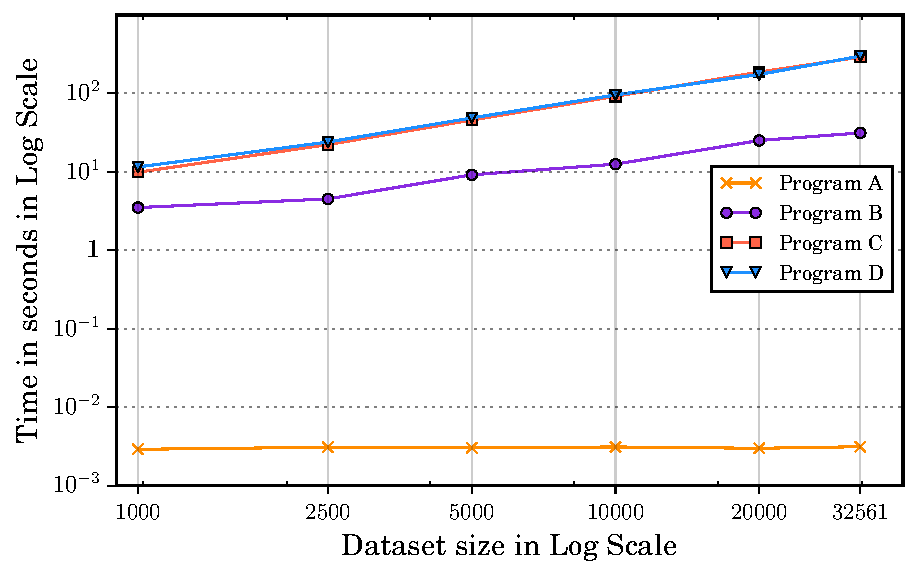
\includegraphics[width=0.6\columnwidth]{scale_final.pdf}
        \caption{\system Program Scalability for 4 programs}\label{fig:scale}
\end{figure}

\begin{figure}[b]
  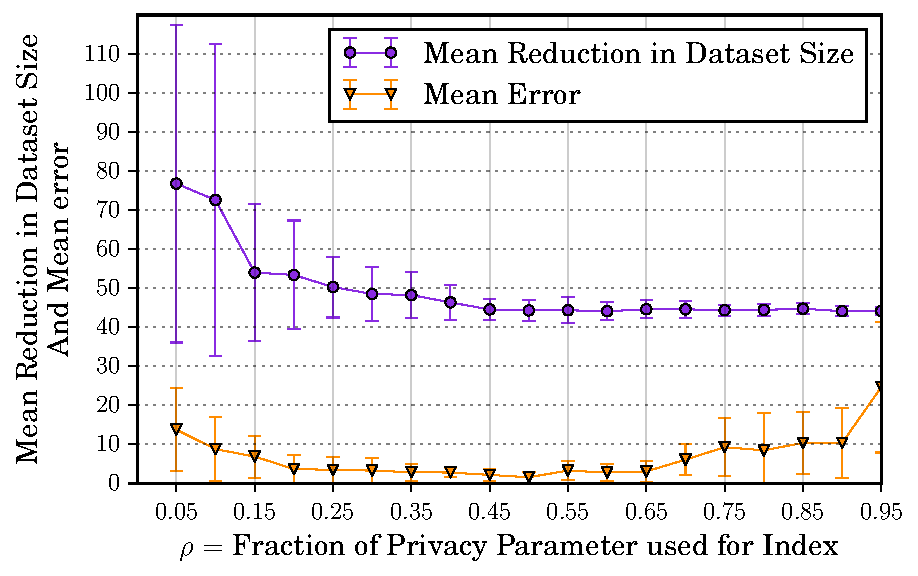
\includegraphics[width=0.6\columnwidth]{index_new.pdf}
  \caption{Accuracy-Efficiency Trade-off in P5 \xh{update}} \label{fig:index_tradeoff}
\end{figure}

\eat{
\begin{subfigure}[b]{0.25\linewidth}
     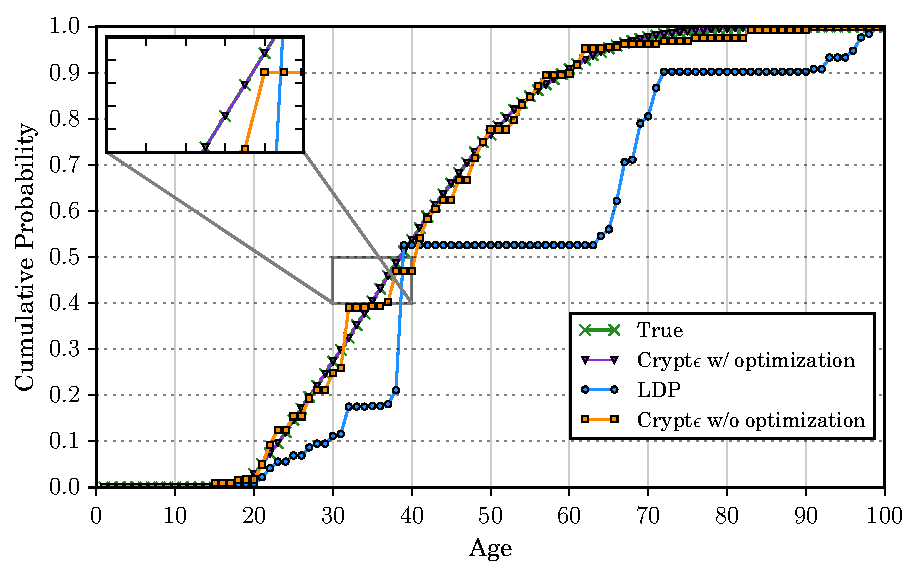
\includegraphics[width=1\linewidth]{cdf_final.pdf}
        \caption{DP Range Tree Evaluation}
        %\label{rangetree}
        \end{subfigure}
}

 %\subsection{Threats to Validity}- 
 %In Table 2 we report the execution time of  the aforementioned $7$ Crypt$\epsilon$ programs. For Program 1 we see that the total time taken for execution for the base case Crypt$\epsilon$ implementation is about 0.5 seconds; the cost is mainly dominated by the \textsf{AS} which has to make a pass through the entire encrypted database. The \textsf{CSP} on the other hand is just needed for decryption in the last step. Program 2 needs to compute the encrypted $Age$ histogram via $GroupBy*$ primitive which takes about $6$ seconds. The \textsf{CSP} time is also more than the previous case because of the garbled circuit in the $NoisyMax$ primitive. The total execution time for the base case implementation for Program 3 is roughly 2 hours.  The reason behind this comparatively higher timing as compared to that of the previous two programs is that the \textsf{CrossProduct} primitive requires  multiplication of the ciphers  which is costlier than the addition operator $\bigoplus$. For Program 4, we observe that the base case implementation takes around 3.1 hours to run. The timing is greater than that for Program 3 because, in this case the additional condition $NativeCountry=Mexico$ results in extra interactions with the \textsf{CSP}. Program 5 requires about $35$ seconds to execute in the base case while Program 6 runs for $41$ minutes. For Program 7 we see that the majority of the time is required by the \textsf{CSP} for generating the encrypted one-hot-codings for the $GroupBy$ primitive and takes $24$ minutes to execute.  An important observation throughout the experiments is that the time taken by the \textsf{AS} is significantly greater than that for the \textsf{CSP} for all the programs except for Program 7. This is a desirable trait for Crypt$\epsilon$ as discussed in section 3.6.



\xh{Remember to add discussion when these optimizations do not help and leave it to future work.}
